\documentclass[a4paper,twoside,12pt]{book}
\usepackage[greek,french]{babel}
\usepackage[T1]{fontenc}
\usepackage[utf8]{inputenc}
\usepackage{fvextra}
\usepackage[xetex]{graphicx}
\usepackage{minted}
\usepackage{hyperref}
\usepackage{setspace}%espacement
\usepackage[margin=3.5cm]{geometry}
\usepackage{setspace}
\usepackage{enumerate,lettrine}
\usepackage[babel]{csquotes}
\usepackage[backend=biber, sorting=nyt, style=enc]{biblatex}
\addbibresource{ref_memoire.bib}
\setlength{\parindent}{1cm}
\onehalfspacing
\hyphenation{}
\hypersetup{
pdfauthor = {Jean Barré},
pdftitle = {mémoire de master 1 HN de l'Ecole des Chartes},
pdfsubject = {measuring literary value},
pdfkeywords = {distant reading} {traitement automatique de la langue} {literary canons}
}


\begin{document}


\frontmatter

\begin{titlepage}
\begin{center}

\bigskip

\begin{large}
UNIVERSITÉ PARIS, SCIENCES \& LETTRES
\end{large}

\begin{center}\rule{2cm}{0.02cm}\end{center}

\bigskip
\bigskip
\bigskip
\begin{Large}
\textbf{Jean Barré}\\
\end{Large}
\begin{normalsize}
\textit{Diplômé de licence mention Lettres}\\
\textit{Diplômé de licence mention Informatique}\\
\end{normalsize}

\bigskip
\bigskip
\bigskip

\begin{Huge}
\textbf{ENTRE CANON ET ARCHIVE, ÉTUDE DES DYNAMIQUES TEXTUELLES À GRANDE ÉCHELLE}\\
\end{Huge}

\bigskip
\bigskip
\begin{LARGE}
\textbf{La valeur littéraire au révélateur des méthodes quantitatives}\\
\end{LARGE}

\bigskip
\bigskip
\bigskip
\vfill

\begin{large}
Mémoire de première année du master\\
\og Humanités Numériques \fg{} \\
\bigskip
2021
\end{large}

\end{center}
\end{titlepage}


\section*{Résumé}
\addcontentsline{toc}{chapter}{Résumé}

Résumé à faire

\medskip

\textbf{Mots-clés: canon ; classique ; archive ; littérature ; textométrie ; humanités numériques ; lecture distante}

\textbf{Informations bibliographiques:} Jean Barré, \textit{Entre Canon et Archive, étude des dynamiques textuelles : La valeur littéraire au révélateur des méthodes quantitatives}, mémoire de master 1 \og Humanités Numériques\fg{}, dir. [Thierry Poibeau, Jean-Baptiste Camps], Université Paris, Sciences \& Lettres, 2021.


\section*{Résumé}
\addcontentsline{toc}{chapter}{Abstract}

abstract

\medskip

\textbf{Keywords: canons ; archives ; literature ; textometry ; digital humanities ; distant reading}

\textbf{Bibliographic Information:} Jean Barré, \textit{Between Canon and Archive, large scale dynamics in the literary field : Literary value assessed by quantitative methods}, M.A. thesis \og Digital Humanities\fg{}, dir. [Thierry Poibeau, Jean-Baptiste Camps], Université Paris, Sciences \& Lettres, 2021.



\mainmatter

\newpage

\tableofcontents

\newpage

\section*{Introduction}
Le mot canon vient du grec ancien \foreignlanguage{greek}{Κανων} qui signifie \og tige de roseau \fg. En littérature, cette étymologie prend tout son sens et donne au canon sa dimension de robustesse, de stabilité. Le canon est une règle, un modèle, une norme à imiter. Il est le fruit d'une hiérarchisation et désigne un ensemble de textes qui font autorité et auquel le monde littéraire fait référence. Les études littéraires s'intéressent à cet ensemble qui ne représente qu'une partie infime de la production littéraire des siècles passés.

Sélectionner des textes est une vieille tradition dans le monde occidental. On peut penser au canon biblique, où une institution, l'Église, instaure une liste de textes formant les Saintes Écritures. Le canon avait alors une valeur d'autorité qui permettait à l'Église de contrôler un récit commun pour la postérité.

Ce modèle de hiérarchisation des oeuvres a été importé en littérature au  \textsc{xix}\ieme ~siècle, à l'époque de la montée des nationalismes, \og quand les grands écrivains sont devenus les héros de l'esprit des nations\fg\footcites{compagnon_demon_2007}. Les critiques littéraires et les universitaires ont hérité de cette tradition en construisant des listes d'auteurs et d'oeuvres qui valaient la peine d'être lues ou introduites dans un processus de recherche. Un exemple symptomatique de la naissance du canon est la parution en 1860 des \og Grands Écrivains de France\fg{} aux éditions Hachette. Dès lors, les éditeurs multiplient les publications des auteurs et des ouvrages susceptibles de leur assurer de larges ventes. 

Le canon est ainsi le résultat d'une longue construction, entre des politiques d'éditions obéissant à une logique de rentabilité économique, une transmission assurée par l'enseignement et une monumentalisation par la critique littéraire. Par ailleurs, si un des rôles de la critique est de juger et de comparer, elle ne peut éviter le processus de canonisation - et de décanonisation - des oeuvres littéraires qu'engendre son activité. Derrière ces critères se trouvent des enjeux esthétiques, idéologiques et institutionnels\footcites{lucken_canon_2019}. En effet, ces listes de classiques sont souvent le reflet d'une représentation idéologisée de l'histoire littéraire qui exclut sauf exception les genres et les ethnies. Le canon littéraire permet malgré tout de simplifier une première approche à la littérature. John Guillory soutient que la formation de listes d'auteurs et d'œuvres permet une distribution du "capital culturel"\footcites{guillory_cultural_1993} dans les écoles, et ainsi réguler l'accès à la littérature, aux pratiques de lecture et d'écriture. Ce qui pose problème dans cette hiérarchisation des textes littéraires est le manque de diversité et d'inclusion dans les listes, comme l'ont montré les recherches récentes sur le sujet \footcites{gonzalez_measuring_2021}.

Le canon littéraire est donc une notion très artificielle, construite avec les biais de la société et modelée par les réceptions successives. L'objectif de ce rapport est de s'extirper d'une analyse politique, historique ou économique de la constitution du canon, et de regarder si les oeuvres canoniques comportent des indices textuels qui leurs sont propres. On peut s'inscrire dans plusieurs démarches pour étudier le canon littéraire. Une approche diachronique consisterait à étudier l'évolution du canon au cours des siècles, en prenant en compte le long processus de mise à jour du canon. Nous allons ici étudier le canon en synchronie, autrement dit en prenant notre temporalité comme point d'ancrage. Nous nous focaliserons sur le canon littéraire qui est parvenu jusqu'à nous et prendrons comme paramètre d'analyse la réception et la constitution contemporaine d'un canon littéraire.

Il s'agit de mettre en lumière l'existence des dynamiques textuelles qui assurent à certaines oeuvres une longévité exceptionnelle et menacent au contraire la transmission d'une majorité d'autres. Une première hypothèse naïve pour expliquer ce phénomène serait de dire que les lecteurs privilégient les textes informatifs aux textes redondants. Cela permet aux premiers de rester imprimés et d'être republiés au fil des années et condamne les seconds à l'extinction. Cette simplification des processus à l'oeuvre dans la formation d'un canon nous permet de rentrer dans les textes et nous donne des éléments quantifiables pour essayer de confirmer ou d'infirmer cette idée reçue. 

L'objectif est d'observer par le biais d'une lecture distante - chère à Franco Moretti\footcites{moretti_graphs_2005} - des tendances historiques qui mettraient au jour des dissimilarités morphosyntaxiques entre deux sous-corpus composés d'une part de romans \og canoniques\fg{} et d'autre part de romans \og non-canoniques\fg. Les méthodes quantitatives nous permettent de traiter des corpus les plus larges possibles, ce qui ouvre la possibilité d'une histoire empirique de la littérature. Dans ce rapport, nous essaierons de reproduire les résultats de l'équipe de recherche du Stanford Literary Lab. Dans leur pamphlet 11\footcites{mark_algee-hewitt_canonarchive_2016} les chercheurs se sont intéressés à la variété lexicale. La première étape de ce rapport consiste à mesurer la quantité de redondances et d'informations présentes dans les deux sous-ensembles de notre corpus.

Après une présentation du corpus et de la démarche quantitative du rapport, nous présenterons , nous terminerons par une analyse quali-quantitative de nos résultats. 


\chapter{Présentation de la démarche quantitative}

\section{Le corpus de travail}
Le corpus du projet \textit{ANR Chapitres}\footnote{\url{https://chapitres.hypotheses.org/}} sera notre base pour cette recherche. Ce corpus est composé de 2968 romans assemblés à partir de ressources trouvées sur internet (wikisource, ebook gratuit, corpus pré-existant sous licence-libre). Il est encodé en XML-TEI, car cela répondait au besoin de structuration des textes pour le projet \textit{ANR chapitres} qui analysait l'évolution de la longueur des chapitres au cours du temps. Comme on peut le voir avec la figure \ref{corpus_bar}, les textes sont bien répartis dans le temps, avec une dominance de la deuxième partie du XIX\ieme ~siècle. 

\begin{figure}[!ht]
    \centering
    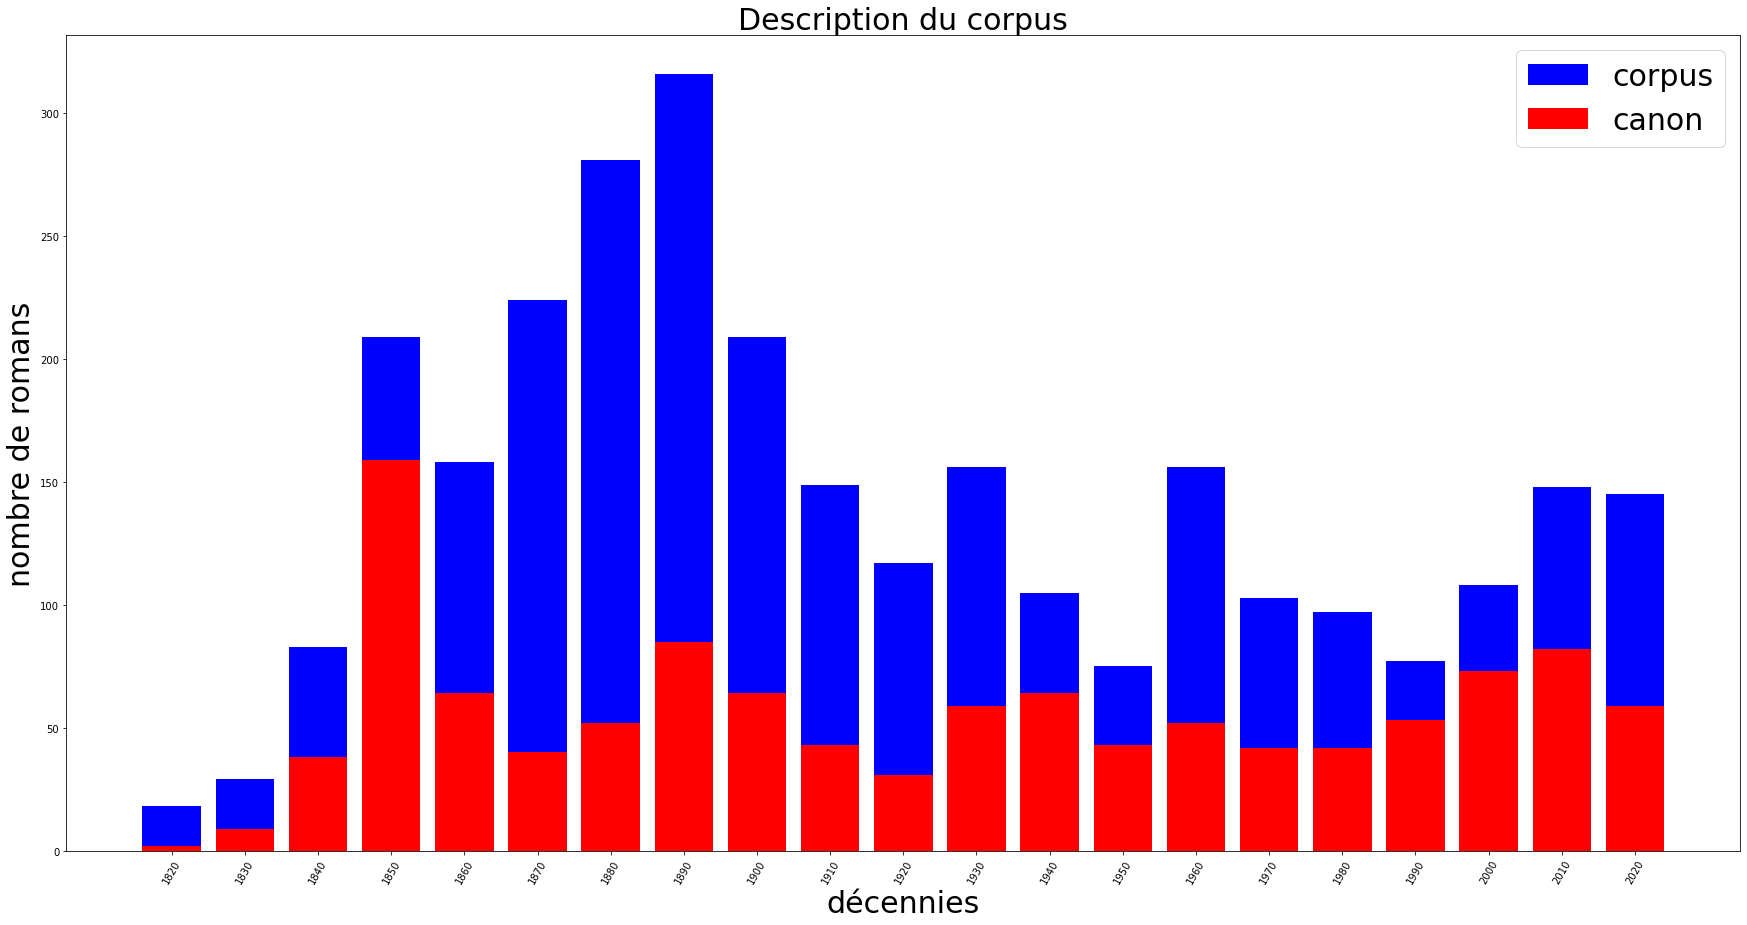
\includegraphics[width=12cm]{img/01_desc_corpus.png}
    \caption{Répartition du corpus dans le temps}
    \label{corpus_bar}
\end{figure}

Le corpus est particulièrement pertinent pour notre étude puisqu'il a été assemblé avec la contrainte de former un équilibre entre les œuvres appartenant ou non au canon. La répartition est de l'ordre de 39\% de romans canoniques et 61\% de non-canoniques comme on peut le constater sur la figure \ref{corpus_bert}.

\begin{figure}[!ht]
    \centering
    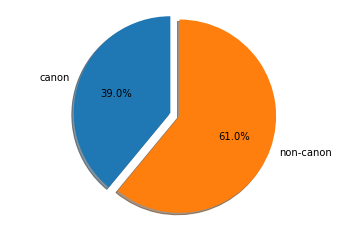
\includegraphics[width=12cm]{img/02_desc_corpus.png}
    \caption{Répartition du corpus entre canon et non-canon}
    \label{corpus_bert}
\end{figure}
\newpage
Le critère utilisé par l'équipe du projet \textit{ANR Chapitres} pour définir l'appartenance ou non d'un texte donné au canon littéraire est le nombre de résultats d'une requête par auteur dans la revue littéraire en ligne Acta Fabula\footnote{\url{https://www.fabula.org/index.php}}. Cela s'inscrit dans la perspective du rapport, qui est d'étudier le canon en synchronie, et plus précisément celui qui est parvenu jusqu'à nous.

\section{Les mesures utilisées}
 Les chercheurs du Stanford Literary Lab se sont intéressés à une mesure linguistique de la variété lexicale, le ratio type-token. La Longman Grammar of Written and Spoken English définit le ratio type-token ainsi : "La relation entre le nombre de formes de mots différentes, ou types, et le nombre de mots courants, ou tokens, est appelée ratio type-token (ou TTR). En pourcentage, le ratio type-token est égal à (types/tokens) * 100".\footcites{biber_longman_2011} Plus il y a de types de lemmes différents, plus la redondance des lemmes et le TTR d'un texte sont faibles, et plus sa variété doit être élevée.

La deuxième mesure utilisée par les chercheurs de Stanford est l'indice de Shannon, qui est tiré de la théorie de l'information\footcites{shannon_mathematical_1948}. Cette dernière est une théorie mathématique de la communication. Cet indice évalue la quantité d'information transmise par les structures linguistiques et l'efficacité de la communication linguistique. De cette manière, Claude Shannon et Warren Weaver cherchaient à mesurer le nombre de bit minimum pour encoder une certaine communication en langage naturel. 

Si l'indice de Shannon a été conçu à l'origine pour mesurer l'entropie, il est devenu un indice très populaire dans divers domaines d'études tels que l'écologie, la géographie et l'anthropologie. Son but est de prédire le type ou l'espèce d'un individu choisi au hasard dans un ensemble de données. Mark Algee-Hewitt propose d'utiliser l'indice de Shannon sur les bigrammes de lemmes\footcites{algee-hewitt_discourse_nodate}. L'indice détermine le contenu informationnel de nos textes en évaluant le degré de prévisibilité de chaque transition de mot à mot, compte tenu de l'éventail des transitions possibles. Ainsi, l'indice de Shannon va nous permettre d'évaluer le niveau de diversité des bigrammes dans chaque roman.

\begin{equation}
H\ensuremath{\prime}=-\sum_{i=1}^R pi ln pi
\end{equation}

La formule est assez simple : R est le nombre de types (ou d'espèces, en écologie), pi est la proportion d'individus pour chaque type dans un échantillon. L'indice de Shannon est connu pour l'importance qu'il accorde à la richesse des espèces (ici des lemmes). On attend dans nos textes que cette mesure soit plus grande pour les canons que pour les archives.

 \section{Les outils du TAL}

Pour quantifier les fréquences d'apparition de mots, on réduit les lexèmes sujets à flexion (les verbes, les substantifs, les adjectifs) à leur unité lexicale commune. On appelle ce processus la lemmatisation. Par exemple, cela permet de compter les différentes formes du verbe être comme autant d'occurrences d'un même lemme, le verbe être. Pour ce traitement, nous utilisons la librairie python Spacy. Cette dernière est très performante pour une analyse sur de grandes quantités de données et couvre tous les traitements d'une chaîne de TAL classique. Cette librairie a aussi l'avantage d'être très bien documentée et comporte plusieurs modèles pour le français. Au vu des performances des différents modèles, nous prenons la décision d'utiliser le modèle fr\_core\_news\_lg qui a un très bon rapport temps d'exécution / performance. Spacy nous permet de tokeniser, lemmatiser et de nettoyer les romans en contrôlant l'étiquetage morphosyntaxique des tokens. Voici la fonction qui va permettre de lemmatiser nos textes avec l'aide de Spacy :

\begin{minted}{python}
def lemmatize(path:str)->list:
    list_lemma = []
    with open(path, encoding="utf8") as file:
        #on récupère l'arbre du document xml
        tree = etree.parse(file)
        #on récupère l'indice de canonicité du roman
        tag = est_canon(tree)
        if tag == True:
            print("canon")
        else:
            print("non_canon")
        #on récupère les paragraphes avec un xpath
        if tree.findall(".//p"):
            for paragraphe in tree.findall(".//p"):
                if paragraphe.text:
                    #on nettoie le texte et on le met dans la pipeline de spacy
                    clean_text = normalize("NFKD", paragraphe.text)
                    docs = nlp(clean_text)
                    for token in docs:
                        #si le token est bien un mot on récupère son lemme
                        if token.pos_ != "PUNCT" and "SPACE" and "X" and "SYM":
                            list_lemma.append(token.lemma_)
    return list_lemma, tag

\end{minted}

On récupère d'abord l'indice de canonicité avec un xpath, puis on récupère le texte qui est encodé dans des balises <p> de paragraphes. On le met dans la pipeline de Spacy qui va tokeniser notre texte, c'est à dire le découper en mots. Ensuite nous contrôlons l'étiquetage morphosyntaxique des tokens avec le Part Of Speech tagging (POS) de Spacy. Cela nous permet de nous assurer que le texte est bien propre : les lemmes récupérés ne sont ni des espaces, ni des chiffres, ni des signes de ponctuation. De cette façon, les calculs réalisés sur ces lemmes seront pertinents. On peut ainsi former des listes de lemmes, ou de n-grams qui seront la base de notre analyse.


\section{Quelques considérations avant l'implémentation}

Avant de lancer les calculs sur notre corpus, il est important de définir les paramètres de nos algorithmes pour que les mesures soient les plus pertinentes possibles. La taille des romans du corpus du projet \textit{ANR Chapitres} varie énormément, entre des nouvelles d'une cinquantaine de pages et des romans fleuves de plus de 3000 pages. Nous avons donc découpé nos textes en morceaux de 1000 mots pour normaliser les mesures. Cela nous a permis de ne pas écraser les résultats des fréquences d'apparition de lemmes ou de bigrammes et de pouvoir comparer les textes entre eux. Pour un texte de 30 000 mots, 30 mesures seront réalisées. Ce n'est qu'après que l'on pourra simplifier nos résultats par une simple moyenne entre les 30 mesures prises. 

En plus de la fenêtre de 1000 mots, nous avons décidé de mesurer l'indice de Shannon sur les 100 bigrammes les plus fréquents de chaque fenêtre. C'est une valeur assez arbitraire néanmoins elle est aussi utilisée par l'équipe de Stanford dans leur publication. 

Après les premières implémentations de l'indice de Shannon sur nos textes, nous avons fait face à un comportement que nous n'avions pas anticipé : La proportion pi d'individus pour les bigrammes de lemmes rares est trop petite (de l'ordre de 10\up{-3}). Le logarithme de cette proportion donne un résultat cohérent mais celui-ci multiplié par cette même proportion donne un résultat du même ordre, insignifiant dans le calcul. Pour simplifier, l'indice de Shannon donne dans notre cas plus de poids à un bigramme redondant qu'à un bigramme rare. Or un bigramme rare améliore le niveau de diversité du passage. Cela devrait faire augmenter par la même occasion l'indice de Shannon.

 On peut expliquer cela par le fait que nos textes possèdent une population de bigrammes très grande (1001 bigrammes par morceaux de 1000 mots) et des fréquences d'apparition très petite. Néanmoins, il nous semblait pertinent de conserver l'indice de Shannon en prenant en compte qu'il ne mesure pas dans notre corpus le contenu informationnel et la diversité mais bien la redondance de second ordre. En d'autres termes, plus l'indice de Shannon est grand, plus les bigrammes de nos textes sont redondants.
 
 
\chapter{Analyse des résultats}

\section{Résultats}

Après avoir lancé les deux algorithmes sur les 2968 romans, des premiers résultats sont générés sous la forme de tableurs de 2968 colonnes. 

\bigskip
\begin{tabular}{cc}
    \centering
    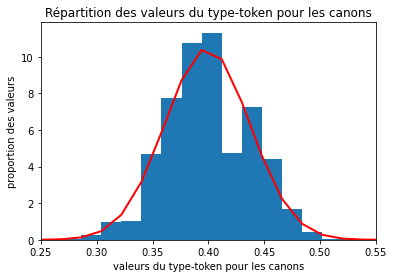
\includegraphics[width=7cm]{img/03_tt_canon_repartition.png} & 
    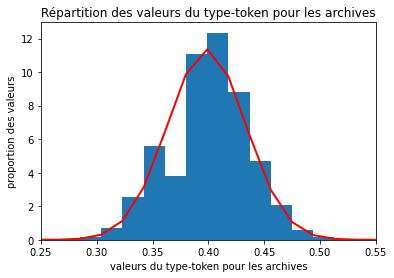
\includegraphics[width=7cm]{img/04_tt_arch_repartition.png} \\ 
    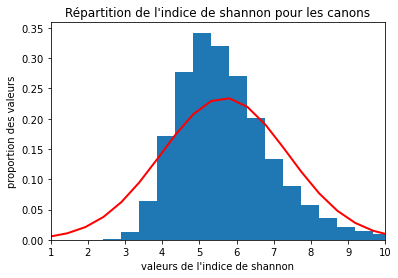
\includegraphics[width=7cm]{img/05_shannon_canon_repartition.png} & 
    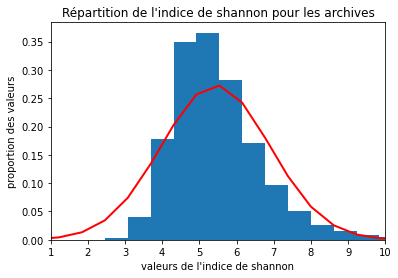
\includegraphics[width=7cm]{img/06_shannon_arch_repartition.png} \\ 
\end{tabular}

 Même si elles ne correspondent pas à une loi normale, nous obtenons une bonne répartition des données pour nos quatre mesures. Ce constat est important car il montre que les valeurs limites portent une signification particulière que nous analyserons dans la suite du rapport.


\subsection{Type-token ratio}
Pour le ratio type-token, un nombre de type de lemme élevé va nécessairement augmenter le résultat, puisque le nombre de token reste le même avec nos fenêtres de 1000 mots. Un type-token élevé implique donc un texte peu redondant et inversement. Nous avons projeté dans la figure \ref{type_token_diagram} nos résultats de cette première mesure sur un graphique avec en ordonnées les moyennes des type-token ratio de chaque roman et en abscisses les années de parutions de nos romans. 

\bigskip
\begin{figure}[!ht]
    \centering
    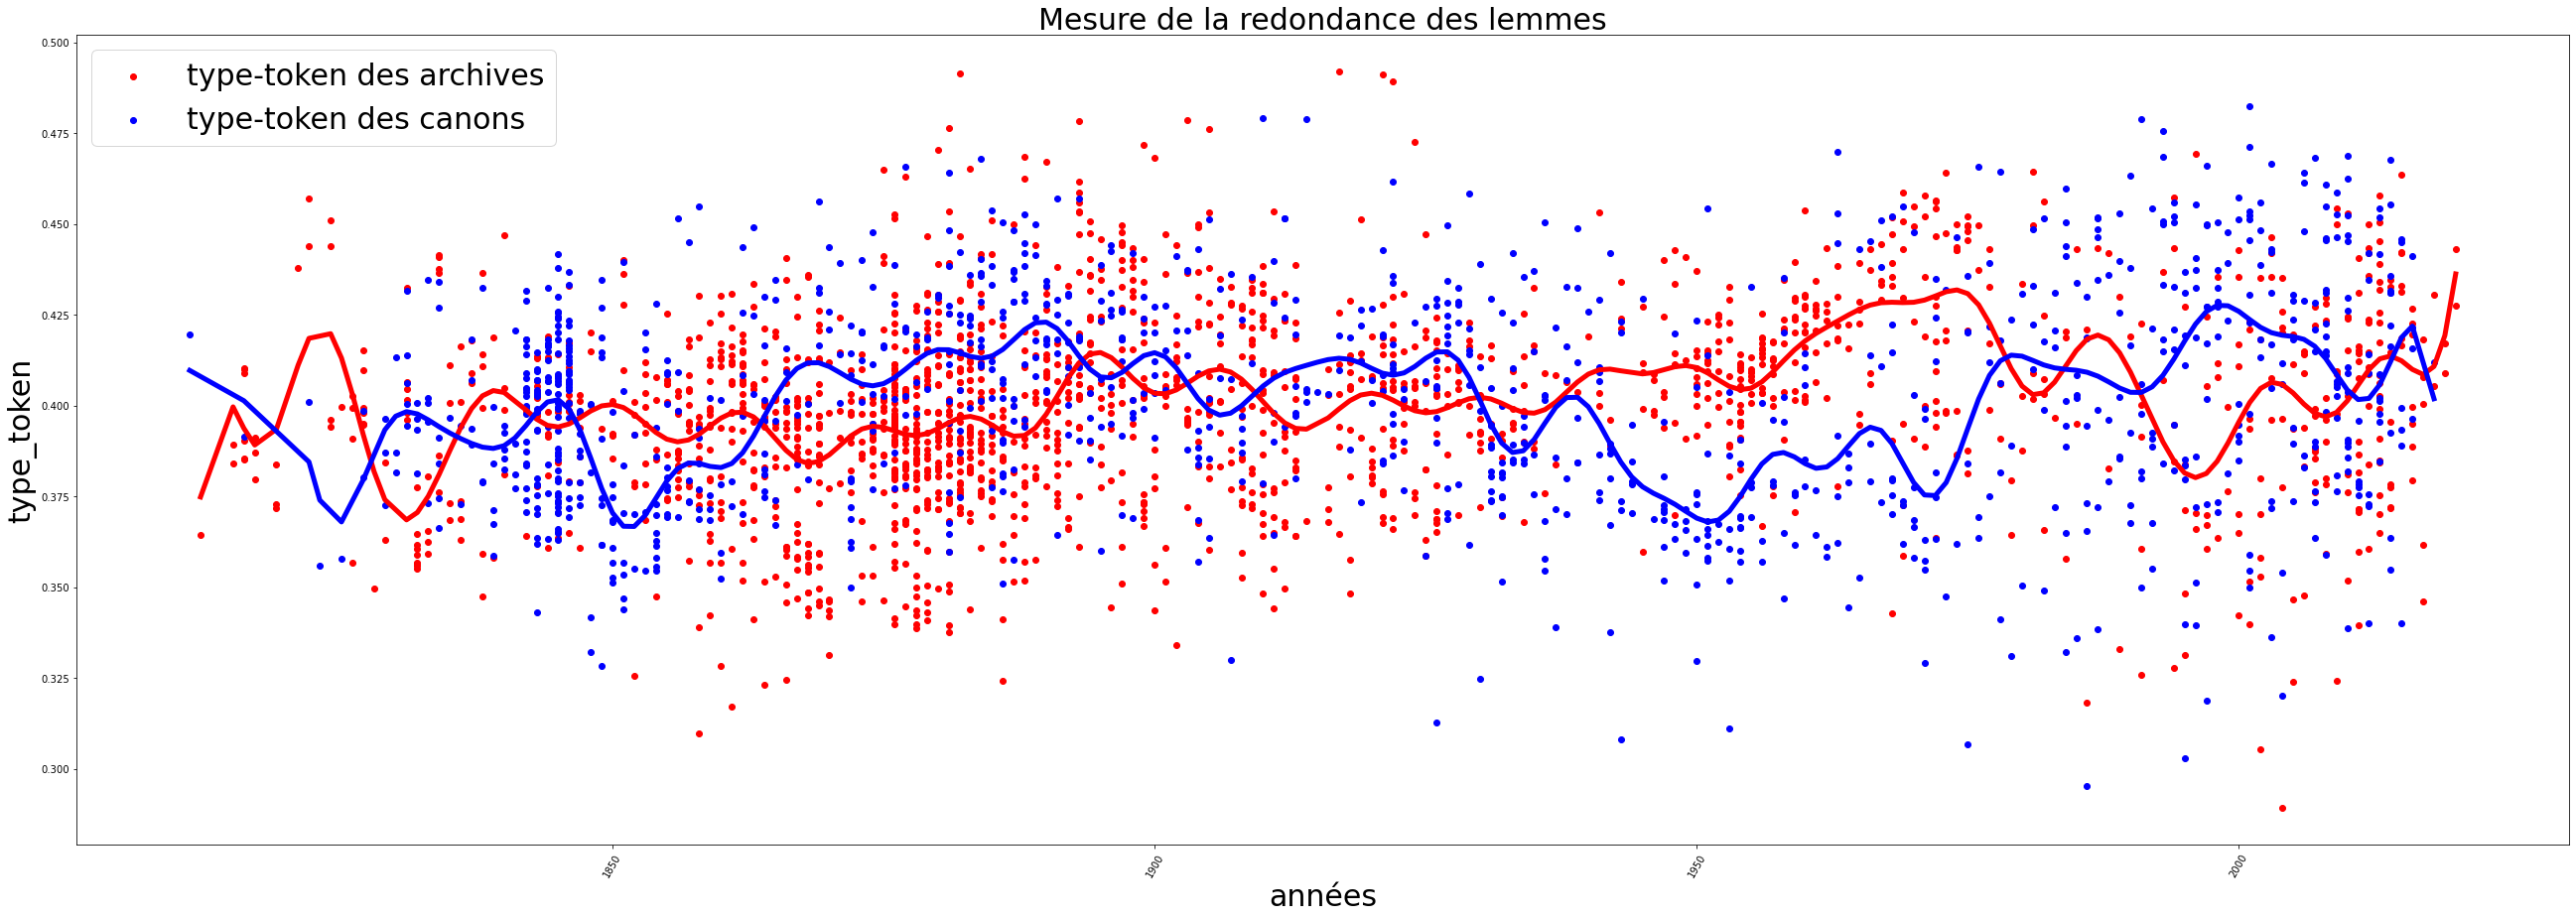
\includegraphics[width=15cm,height=7cm]{img/07_results_type_token_regression.png}
    \caption{Fréquence d'apparition des lemmes}
    \label{type_token_diagram}
\end{figure}

Pour rendre plus lisibles les résultats, nous avons implémenté une régression non-linéaire qui trace la moyenne ajustée aux valeurs de proche en proche. La figure \ref{type_token_diagram} représente donc la redondance des lemmes au cours du XIX\ieme ~et du XX\ieme ~siècle dans les romans du corpus \textit{ANR Chapitres}. S'il n'y a pas de tendance qui se dégage entre nos deux sous-corpus au XIX\ieme ~et dans la première moitié du XX\ieme ~siècle, on remarque que nos données se séparent en deux groupes distincts aux alentours des années 1940 puis se rejoignent dans les années 1980. Ces quarantes années correspondent aussi à un minimum local très marqué pour nos romans canoniques. On peut en effet constater une baisse du type-token ratio et donc une augmentation de la redondance sur cette période. Pour vérifier notre première impression, nous avons effectué avec la figure \ref{boxplot_tt} un diagramme en boîte en sélectionnant la période 1940-1980.

\bigskip
\begin{figure}[!ht]
    \centering
    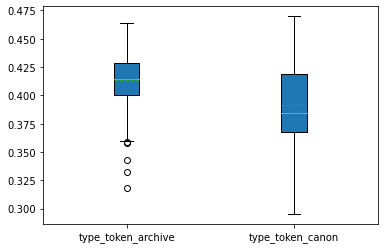
\includegraphics[width=10cm]{img/08_boxplot_type_token.png}
    \caption{diagramme en boîte sur la période discriminante pour le ratio type-token}
    \label{boxplot_tt}
\end{figure}

Sur cette période donnée, nos archives sont d'une part beaucoup plus concentrées que nos canons et d'autre part les résultats sont plus élevés pour nos archives que pour nos canons. Le rectangle bleu des archives, qui correspond à 50\% des valeurs (du premier au troisième quartile) se place au dessus de la médiane de celui des canons. Il y a donc une différence notable sur cette période.

\subsection{Indice de Shannon}

Grâce à l'indice de Shannon, l'équipe de Stanford a trouvé des différences significatives entre les deux sous-corpus. Dans notre cas, la différence entre canon et non-canon n'est pas aussi marquée. Comme on le voit sur la figure \ref{bigram_shannon}, les deux régressions qui tracent la moyenne de proche en proche, pour les canons en bleu et pour les archives en rouge, sont très homogènes. Cependant, nous retrouvons la même période discriminante que la figure \ref{type_token_diagram} du type-token ratio. Sur cette période, si les mesures pour les archives restent cohérentes avec le siècle passé, celles pour les canons augmentent rapidement et marquent un plateau d'une cinquantaine d'années. 

\bigskip
\begin{figure}[!ht]
    \centering
    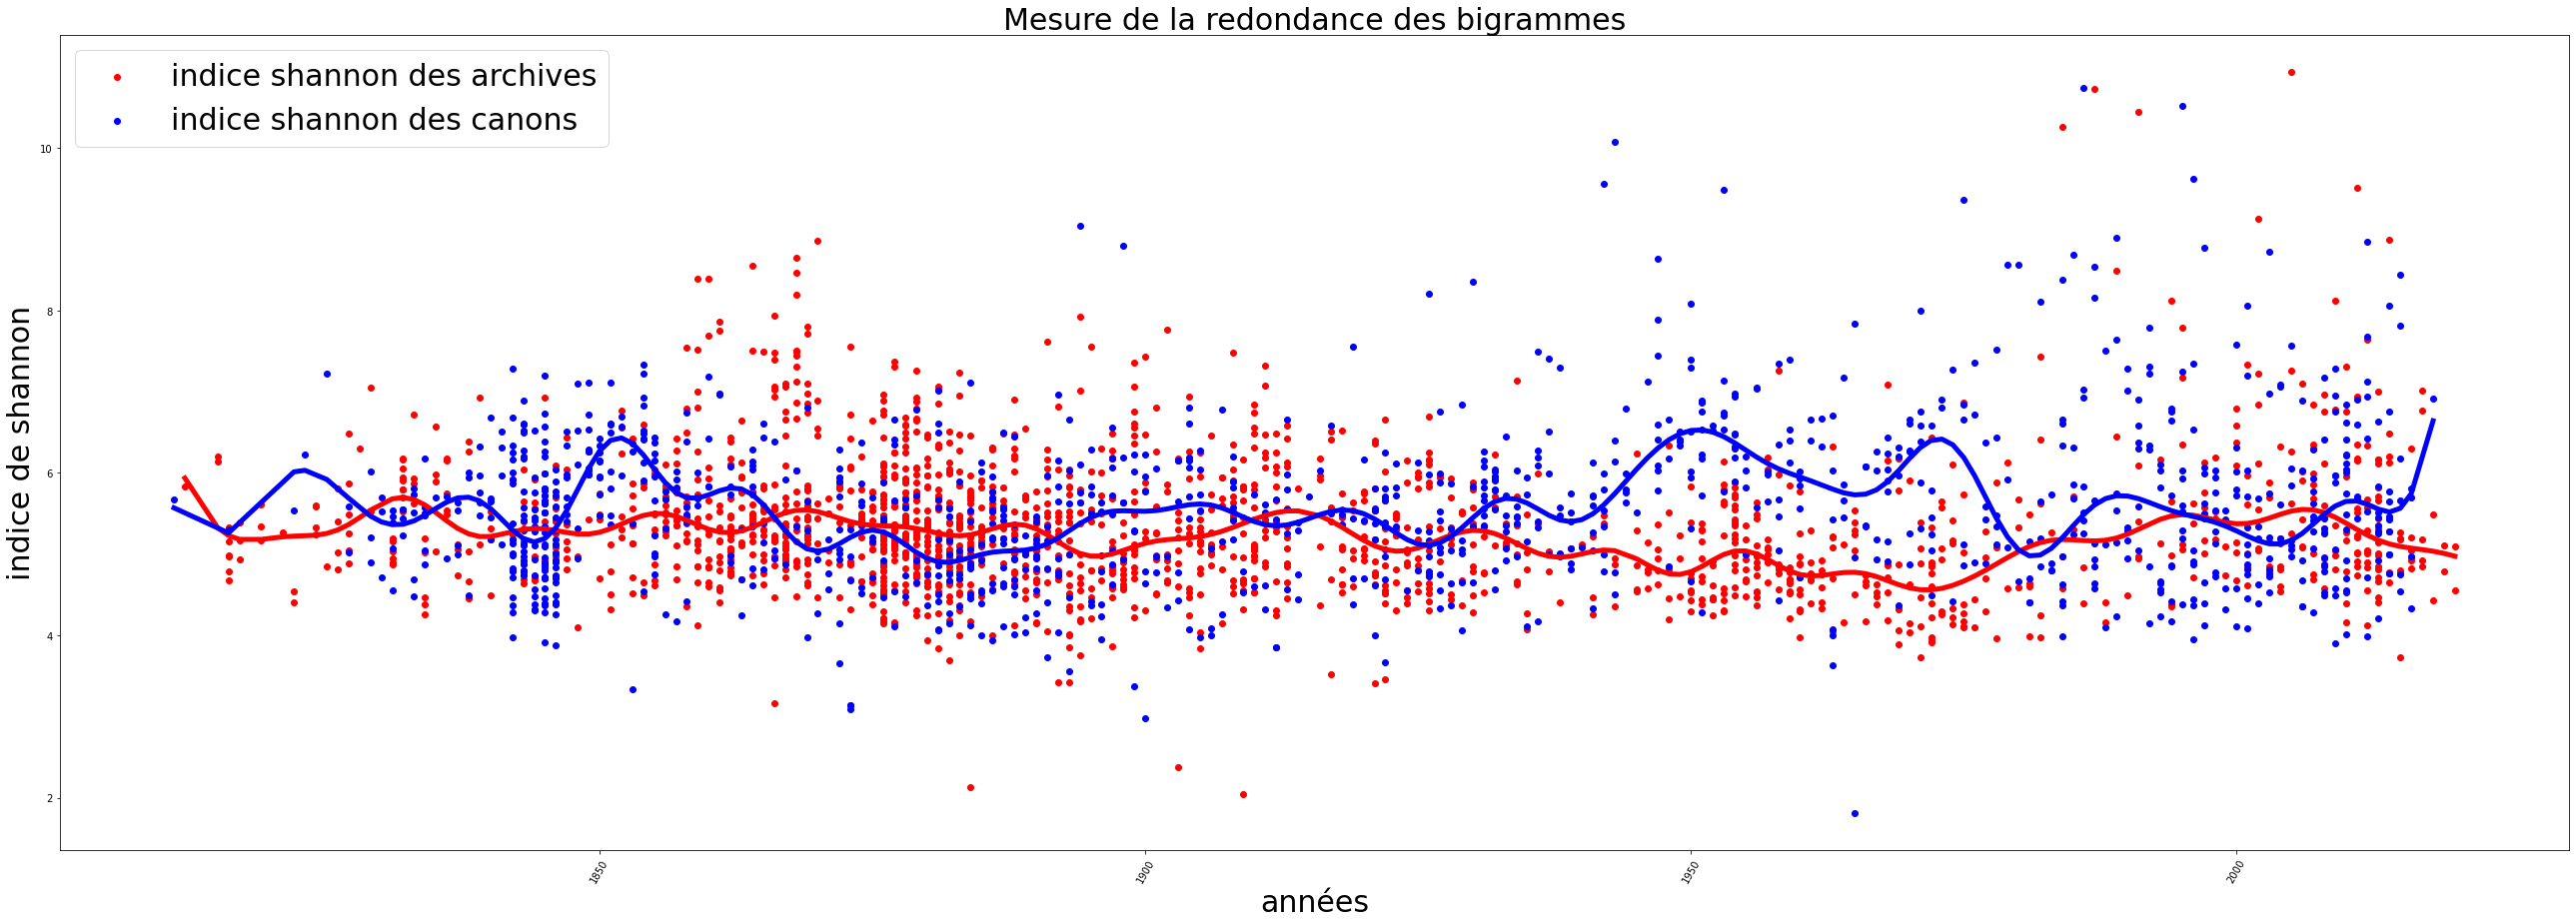
\includegraphics[width=15cm,height=7cm]{img/09_results_shannon_regression.png}
    \caption{Mesure de la redondance des bigrammes}
    \label{bigram_shannon}
\end{figure}

Pour confirmer cette analyse, nous avons réalisé un diagramme en boîte en figure \ref{boxplot_sha} pour les mesures de Shannon sur la période de 1940 à 1990. Il se trouve que 50\% des valeurs des romans canoniques dominent le troisième quartile des archives. Nous retrouvons ainsi le même phénomène que pour la mesure du type-token ratio.

\bigskip
\begin{figure}[!ht]
    \centering
    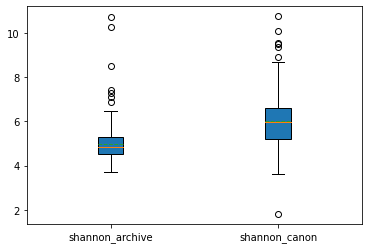
\includegraphics[width=10cm]{img/10_boxplot_shannon.png}
    \caption{diagramme en boîte sur la période discriminante pour l'indice de Shannon}
    \label{boxplot_sha}
\end{figure}

C'est un constat intéressant qui conforte les premiers résultats. Il y a dans la deuxième partie du XX\ieme~ siècle un niveau de redondance des lemmes et des bigrammes qui sort de l'ordinaire pour nos romans canoniques. 

\section{Analyse des résultats}

Les romans classifiés comme canoniques dans le corpus \textit{ANR Chapitres} sont donc plus redondants que les archives sur une période d'environ 50 ans. C'est un résultat auquel on ne s'attendait pas, puisque notre hypothèse de départ penchait vers le contraire. Maintenant que nos résultats montrent ce phénomène, il est légitime de se demander pourquoi le type-token ratio et l'indice de Shannon séparent si bien nos romans ? Et pour quelles raisons sur cette période donnée en particulier ? Il est assez compliqué de répondre à ces questions sans revenir vers une analyse qualitative, mais on peut trouver des éléments de réponses dans la littérature scientifique sur les fréquences de mots dans les romans.

En effet, les travaux de Susan Conrad et de Douglas Biber\footcites{biber_register_2019} montrent que les résultats du type-token ratio diffèrent selon les registres utilisés dans le texte. L'opposition fondamentale se situe entre l'oral et l'écrit, avec un rapport type-token plus élevé pour l'écrit que pour l'oral. Cela s'explique en partie par le niveau de langue, qui est plutôt soutenu dans les textes littéraires et familiers ou communs dans les discours rapportés. Plus précisément, Susan Conrad et de Douglas Biber ont travaillé sur de vastes corpus d'anglais parlé et écrit dans quatre registres ; conversation, fiction, nouvelles et prose académique. Ils caractérisent la conversation comme étant co-construite par deux ou plusieurs locuteurs, qui adaptent de manière dynamique leurs expressions à l'échange en cours. Les locuteurs répètent souvent ce qui a été dit, que ce soit pour relier des concepts, focaliser l'attention ou simplement gagner du temps de réflexion. Ainsi, selon cette étude, la conversation serait nettement plus répétitive que les trois autres registres écrits qu'ils examinent.

Mais si l'archive présente donc une plus grande variété lexicale que le canon, ce n'est pas forcément qu'elle tend vers un registre plus "écrit" que le canon. En effet les travaux de Marissa Gemma, Frédéric Glorieux et Jean-Gabriel Ganascia sur les discours familiers\footcites{gemma_operationalizing_2015} montrent que la répétition est aussi une caractéristique du discours familier dans les romans :
\begin{displayquote}
 Au fur et à mesure que nous avançons dans le 20e siècle, et que la répétition de mots et de phrases devient une caractéristique plus importante du discours romanesque, les répétitions deviennent aussi nettement plus familières ; cette tendance est parfaitement illustrée par la façon dont les personnages romanesques en viennent à s'adresser et à se référer les uns aux autres en se tutoyant.
\end{displayquote}
Dans notre graphique du type-token ratio, nous retrouvons cette tendance observée par Marissa Gemma, Frédéric Glorieux et Jean-Gabriel Ganascia. Les romans entre 1940 et 1980 sont très redondants par rapport au siècle précédent. Cela pourrait donc s'expliquer par une utilisation plus prononcée dans nos canons de l'oralité et de la familiarité.

\chapter{Recherches de conjectures}

\section{Les valeurs aberrantes}

Il faudrait maintenant repérer dans le corpus les romans les plus caractéristiques de nos résultats, en repérant par exemple les valeurs "aberrantes" du type-token ratio ou de l'indice de Shannon. Une lecture qualitative sur les passages et les romans les plus redondants pourraient infirmer ou confirmer nos hypothèses sur la présence du registre familier et des paroles rapportées pour expliquer ce niveau de redondance de la variété lexicale. 

\subsection{A l'échelle des morceaux de texte}
En filtrant nos résultats, nous obtenons les passages limites du corpus. 
Le passage le moins redondant (celui avec la mesure du type-token ratio la plus grande) se trouve chez Georges Perec, dans un recueil posthume de textes intitulé \og\textit{Cantatrix sopranica L}\fg{} publié en 1991. Ce dernier compile des pseudo-études scientifiques ou littéraires. Le passage qui nous intéresse obtient un ratio type-token de 61\%, ce qui est remarquable puisque la moyenne du corpus est d'environ 40\%.

\bigskip
\begin{figure}[!ht]
    \centering
    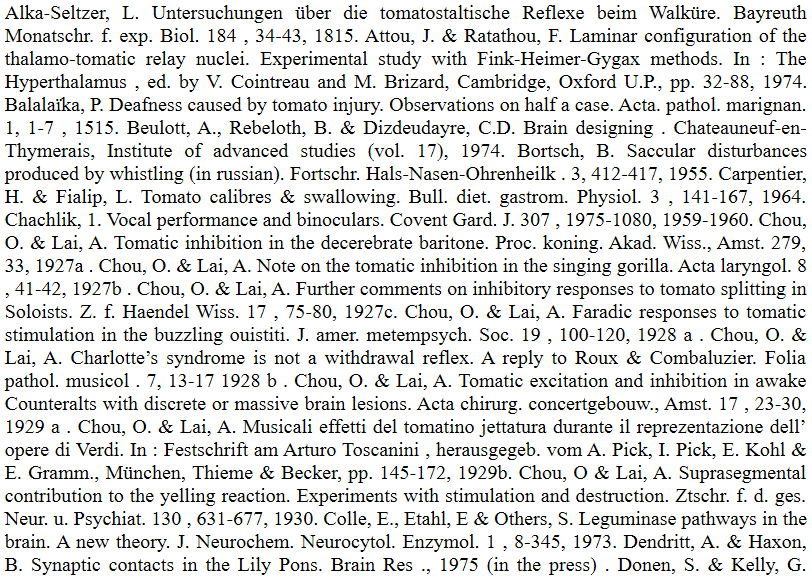
\includegraphics[width=10cm]{img/11_passage_tt_grand.png}
    \caption{Passage avec le TTR le plus grand du corpus}
    \label{cantatrix}
\end{figure}
\bigskip

Comme on peut le voir dans la figure \ref{cantatrix}, le passage en question est la bibliographie de l'article scientifique parodique. Le nombre de type très élevé s'explique par la présence de nombreux noms propres différents dans les références. Un autre élément important est qu'il n'y a presque pas de connecteurs logiques ni de mots outils. 

Le passage le plus redondant (celui avec la mesure du type-token ratio la plus petite) vient du roman \textit{L'Innommable} de Samuel Beckett publié en 1953. C'est un roman très particulier qui s'inscrit dans la lignée des oeuvres de Beckett et de son travail sur l'absurdité de la condition humaine. Il n'y a pas d'intrigue, seulement une suite de digressions autour du néant. Le type-token ratio de ce passage est de 16\%, la figure \ref{innommable} en montre un extrait.

\bigskip
\begin{figure}[!ht]
    \centering
    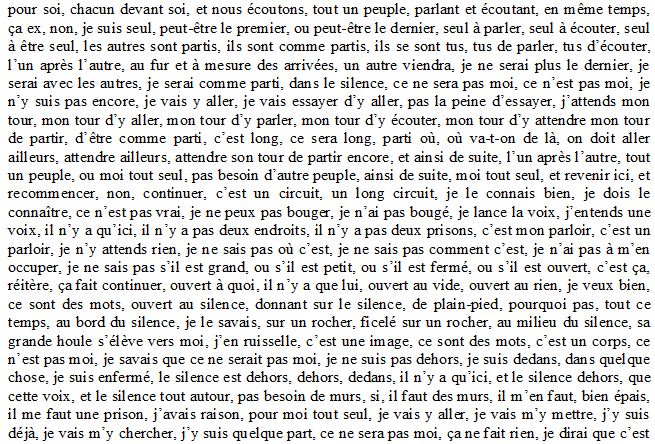
\includegraphics[width=10cm]{img/12_passage_tt_petit.PNG}
    \caption{Passage avec le TTR le plus petit du corpus}
    \label{innommable}
\end{figure}
\bigskip

Le roman est un flux de pensées ininterrompues. En effet, Samuel Beckett va très loin dans la représentation de la parole intérieure. L'état psychologique du narrateur est montré sans filtres et sans vouloir correspondre aux conventions littéraires. On assiste au délitement de l’intériorité du narrateur, qui perd contrôle sur lui-même et ses pensées. Le narrateur répète ses mots mais aussi des structures de phrases entières, ce qui renforce la redondance. Le registre familier est ici utilisé, mais il n'explique pas à lui seul la redondance élevée du roman. En effet, le type-token ratio est sensible au traitement de la parole intérieure, d'autant plus quand elle est hors de contrôle et débridée. Le passage est uniquement au discours direct libre. Par ailleurs, on a montré que l'oralité était un facteur fondamental dans la baisse de la variété lexicale. Cela se confirme dans ce passage précis, construit entièrement sur des paroles rapportées. 

L'indice de Shannon met en avant tous les passages d'un ouvrage en particulier. Il s'agit de \textit{Je me souviens} de Georges Perec. C'est un recueil de bribes de souvenirs de la vie de l'auteur. L'ouvrage est construit sur une anaphore de \og Je me souviens\fg au début des 480 fragments. On peut en voir un extrait avec la figure \ref{jemesouviens}.
\bigskip
\begin{figure}[!ht]
    \centering
    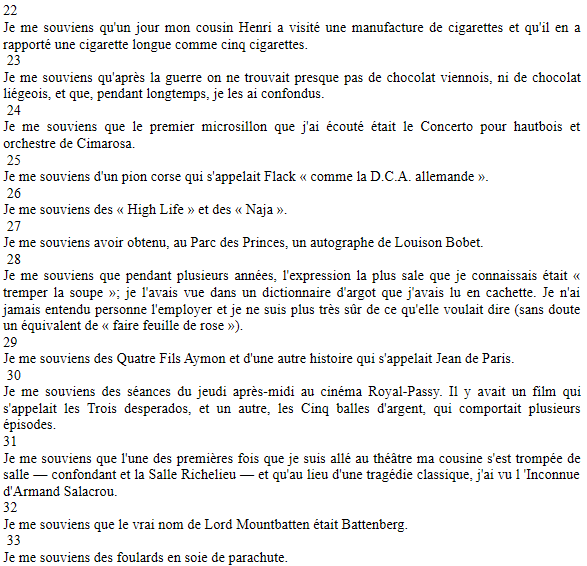
\includegraphics[width=10cm]{img/13_passage_shannon_grand.png}
    \caption{Passage le plus redondant du corpus}
    \label{jemesouviens}
\end{figure}
\bigskip

Notre calcul de l'entropie souligne à quel point la liaison d'un mot à un autre est prévisible et les résultats pour les passages de \og Je me souviens\fg sont 6 à 7 fois plus importants que pour le reste de notre corpus. Les bigrammes de l'anaphore \og Je me\fg \og me souviens\fg et \og souviens que\fg réalisent à eux seuls des scores importants. Les résultats du type-token ratio sont eux dans la moyenne, ce qui montre bien que c'est la construction des phrases qui est remarquée ici.

\subsection{A l'échelle des ouvrages}

Pour tenter de comprendre à plus grande échelle de quelle nature sont faits les romans redondants, on peut essayer de compiler nos deux mesures pour faire l'exégèse des cas limites Pour cela, on projette sur un graphique l'ensemble des romans en fonction de leurs moyennes de l'indice de Shannon ainsi que du type-token ratio.

\bigskip
\begin{figure}[!ht]
    \centering
    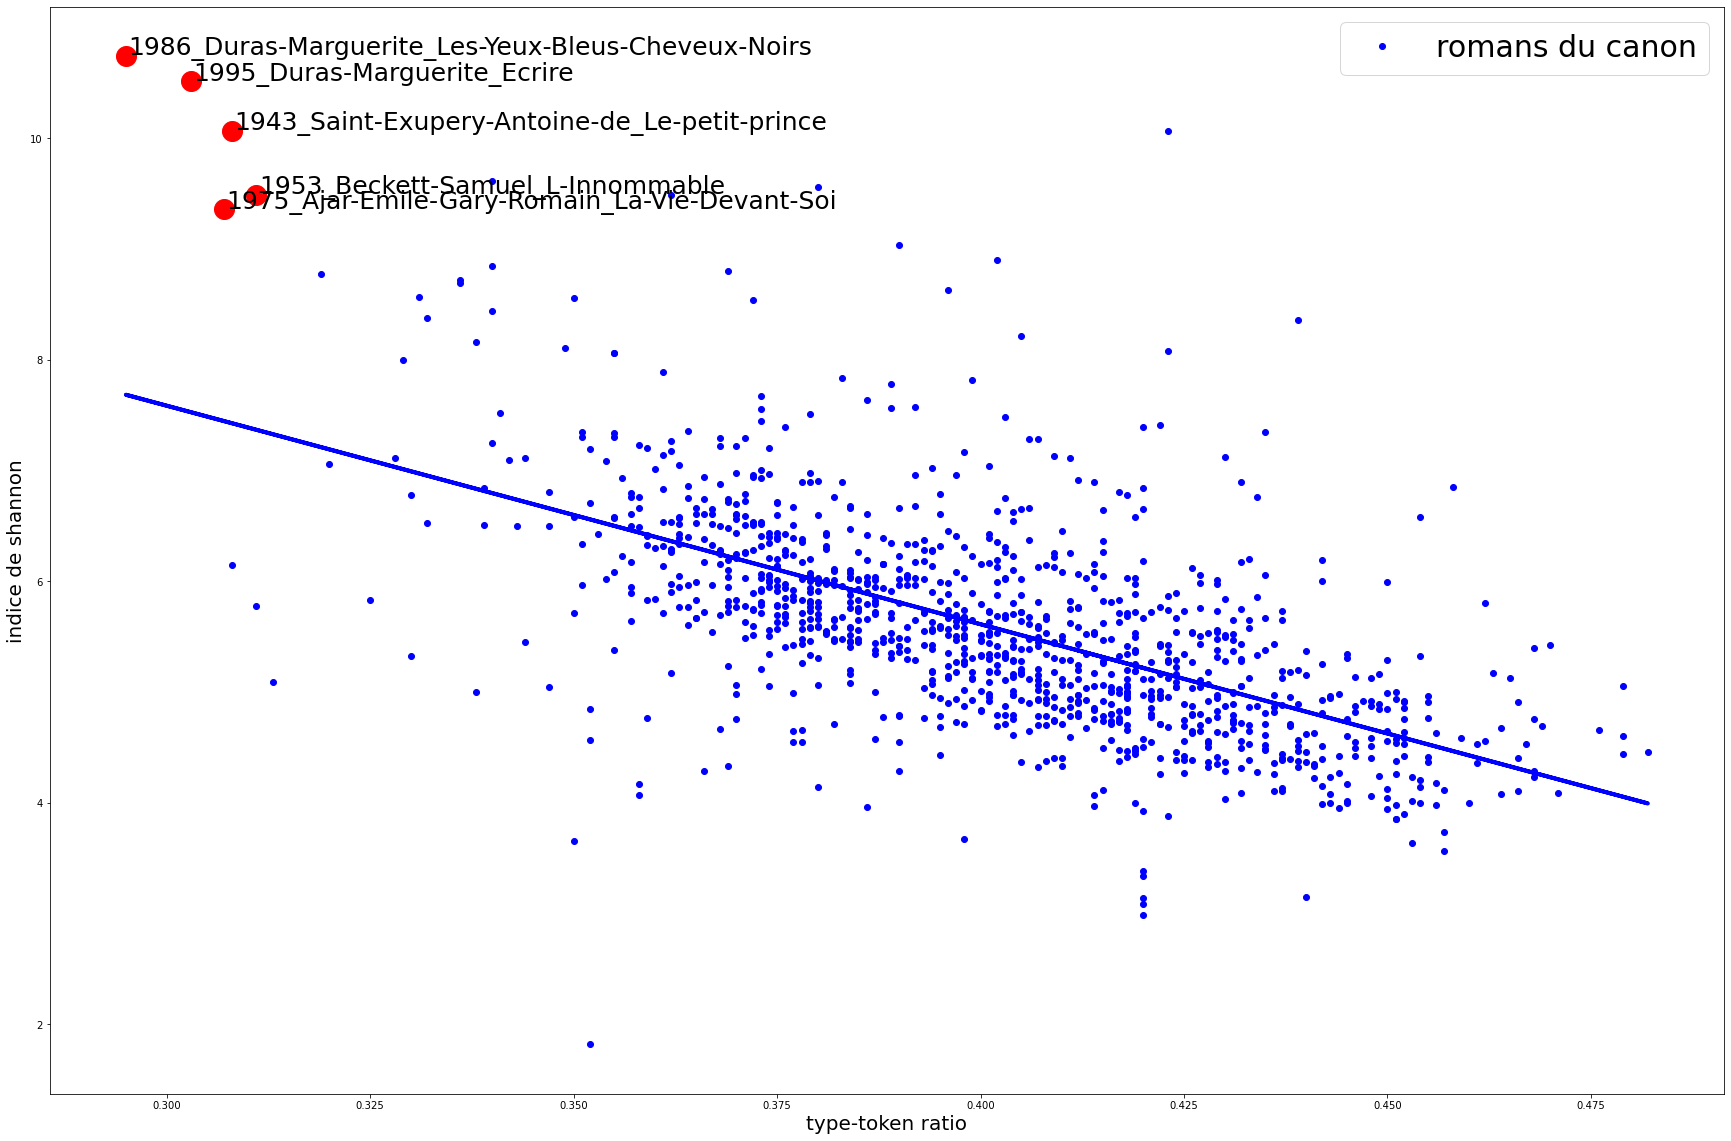
\includegraphics[width=10cm]{img/14_canons_redondants.png}
    \caption{Redondance des romans canoniques}
    \label{canonsredondants}
\end{figure}
\bigskip

La figure \ref{canonsredondants} montre une corrélation entre nos deux mesures, ce qui est logique puisqu'elles calculent chacune à leur manière la redondance dans les textes. Les textes possédant un résultat pour l'indice Shannon très grand ainsi qu'un type-token ratio très faible sont les plus redondants du corpus. La figure \ref{canonsredondants} désigne cinq romans très redondants : il s'agit de \og\textit{Le Petit Prince}\fg{} d'Antoine de Saint-Exupéry, \og\textit{L'Innommable}\fg{} de Samuel Beckett, \og\textit{Écrire}\fg{} et \og\textit{Les yeux bleus cheveux noirs}\fg{} de Marguerite Duras et enfin \og\textit{La Vie Devant Soi}\fg{} d'Émile Ajar.

On remarque que les cinq ouvrages appartiennent à la période discriminante (1940-1990) vue en figure \ref{type_token_diagram} et \ref{bigram_shannon}. Ces cinq ouvrages sont donc les plus symptomatiques de cette période. Pour autant, il n'est pas facile de mettre au jour une unité littéraire tangible entre ces cinq romans. Le premier est une œuvre poétique et philosophique sous l'apparence d'un conte pour enfants. Le deuxième pose des questions existentielles et traite de la contingence de la condition humaine. Le troisième et le quatrième sont deux ouvrages très différents de Marguerite Duras. \og\textit{Écrire}\fg{} est une compilation des tenants et aboutissants du métier d'écrivain, tandis que \og\textit{Les yeux bleus cheveux noirs}\fg{} est un roman sur la passion et la fascination : toute l’intrigue se fonde sur un traumatisme intérieur que le récit ne peut que suggérer par ses répétitions et ses silences, ses images obsédantes, ses ruptures énonciatives. Enfin, \og\textit{La Vie Devant Soi}\fg{} est un portrait sombre d’un enfant immigré orphelin. Nos cinq romans sont donc trop différents pour conclure sur des changements potentiels dans la nature des textes et dans la manière de faire littérature à cette période. 

\section{Conjectures sur cette hausse de redondance}

Si l'on met en perspective nos résultats avec le contexte historique et les remous de la théorie littéraire on peut commencer à comprendre les enjeux de cette époque donnée. Tout d'abord, il faut signaler que cette hausse de la redondance dans nos textes s'effectue à la fin des années 1940, aux lendemains de la seconde guerre mondiale. Les remous de cette période sont illustrés par l'affirmation en 1949 de Theodor Adorno \og Écrire un poème après Auschwitz est barbare\fg\footcites{adorno_prismes_2003}. Par cette formule cinglante, ce dernier refuse l'amnésie collective d’une \og culture  ressuscitée\fg{} et appelle à la prise de conscience de l’enjeu métaphysique que représente la rupture radicale de la Shoah, qui constitue une négation de l’humanité par elle-même. La période est ainsi marquée par une remise en question de tous les champs culturels. 

En littérature, les critiques et les écrivains cherchent à rénover le roman en s'affranchissant des règles de composition dramatique et des objectifs didactiques du roman balzacien\footcites{labouret_litterature_2013}. Le renouveau de la critique littéraire française, emmené par les structuralistes Roland Barthes et Gérard Genette, bouleverse la théorie littéraire. Des thèses comme la mort de l'auteur\footcites{barthes_bruissement_2015} ou le degré zéro de l'écriture\footcites{barthes_degre_1972} remettent en cause les conceptions ancestrales de la littérature. Barthes rend au texte toute sa vivacité et le soustrait de l'emprise de la figure paternelle de l'auteur pour faire place aux interprétations successives des lecteurs. Ce renouveau critique crée un climat propice à la création de nouvelles formes littéraires. C'est dans ce contexte qu'est publié \og Pour un nouveau roman\fg\footcites{robbe-grillet_pour_2013}, où Alain Robbe-Grillet résume les motivations du monde littéraire de l'époque. Robbe-Grillet décline les \og notions périmées\fg{} dont il faut faire selon lui table rase : le  personnage, l’histoire, la forme et le contenu. Les auteurs de ce courant refusent en effet la caractérisation psychologique des personnages et l’histoire perd toute organisation logique et chronologique. Les auteurs s'en remettent à un lecteur actif, qui comble les blancs du récit et participe à la construction du sens. Se constitue alors un courant littéraire, Le Nouveau Roman, qui inscrit le roman dans une dynamique créatrice de possibilités, repoussant les conventions du roman traditionnel tel qu'il s'était imposé depuis le XIX\ieme siècle. Les auteurs de ce courant très particulier ont tous publié chez le même éditeur, les Éditions de Minuit. Notre corpus dispose d'une partie de ces auteurs : Alain Robbe-Grillet, Claude Simon, Samuel Beckett et Nathalie Sarraute. Nous pouvons comparer leurs oeuvres avec le reste du corpus, pour regarder si ce mouvement littéraire a un impact sur les mesures de variétés lexicales que l'on a mené dans ce rapport. La figure \ref{nouveauxromans} met en lumière la place qu'occupe les ouvrages du Nouveau Roman dans la redondance de notre corpus canonique.

\bigskip
\begin{figure}[!ht]
    \centering
    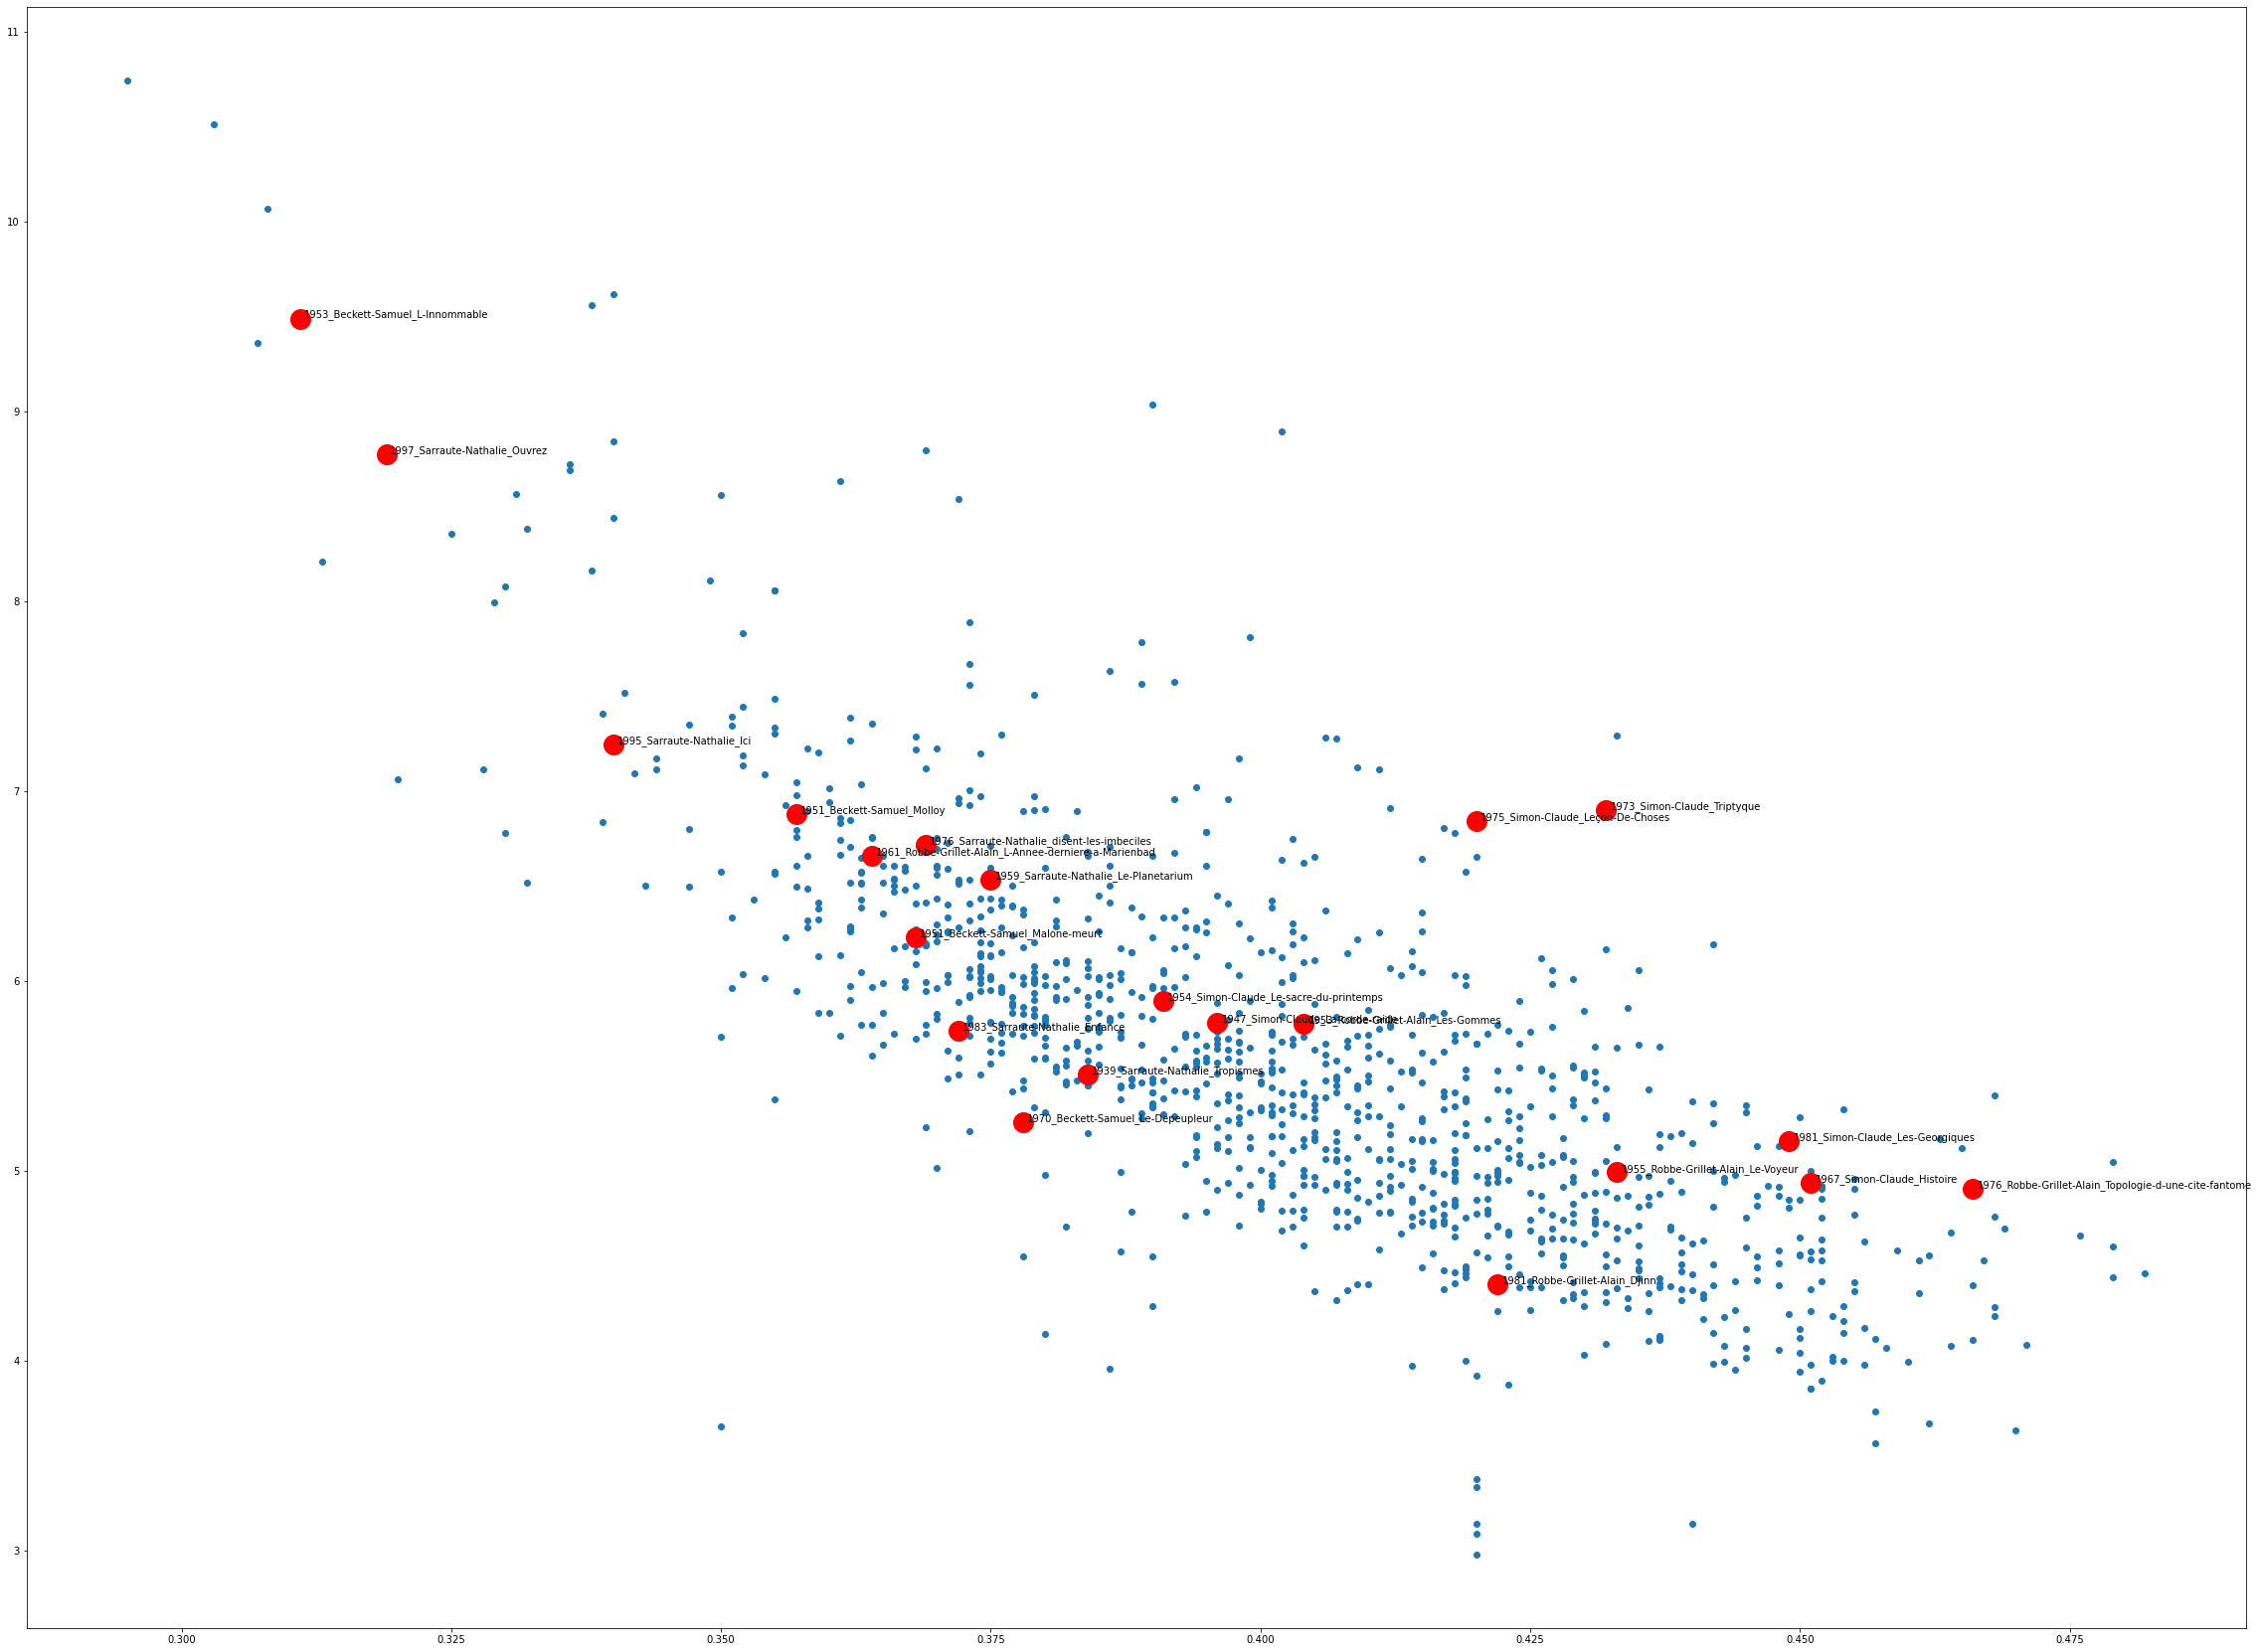
\includegraphics[width=10cm]{img/15_nouveau_roman.png}
    \caption{Redondance dans le Nouveau Roman}
    \label{nouveauxromans}
\end{figure}
\bigskip

Il est intéressant de constater que les résultats de notre analyse sur la redondance lexicale parviennent à capter les remous de cette période. Les ouvrages du Nouveau Roman obtiennent pour la plupart des résultats de redondance assez importants. Ils se placent dans la partie redondante du sous-corpus canonique, même s'ils ne se démarquent pas totalement. On peut conjecturer que l'émancipation des formes plus classiques du roman entraîne une augmentation de l'emploi de niveaux de langue différents, et une nouvelle liberté sur la retranscription des paroles intérieures. L'augmentation de la redondance repérée en figure \ref{type_token_diagram} et \ref{bigram_shannon} dans nos textes canoniques sur la période 1940-1990 trouverait son explication avec le renouveau littéraire qu'apporte le Nouveau Roman. 

Il faudrait étoffer ces premiers résultats avec d'autres analyses. Quantifier les différences qu'apporte le Nouveau Roman dans la sphère littéraire n'est pas une chose aisée, et ce travail ouvre simplement une possibilité de recherche plus avancée sur ce sujet. La mesure de la variété lexicale introduit une problématique connue de la critique mais jamais vérifiée empiriquement. 

\newpage

\section*{Conclusion}
Pour conclure, l'implémentation de méthodes quantitatives nous a permis d'augmenter la focale pour percevoir des tendances historiques. Le choix de mesurer la redondance 


résultats auxquels on ne s'attendait pas forcément. L'hypothèse de base était fondée sur un lieu commun de la littérature qui est de dire que les lecteurs privilégient les textes informatifs aux textes redondants. Cela s'est révélé ne pas être pertinent sur notre corpus, et l'hypothèse est probablement fausse vu notre approche empirique. Nos résultats étaient donc homogènes, tant la mesure du ratio type-token que celle de l'indice de Shannon. Néanmoins, une période d'une cinquantaine d'année a retenu toute notre attention. Les ouvrages canoniques se trouvaient être plus redondants que les non canoniques au lendemain de la seconde guerre mondiale. Nous avons donc cherché ce que montraient véritablement nos mesures sur nos morceaux de textes avant d'essayer de trouver des réponses à l'échelle des oeuvres. Si on peut expliquer l'augmentation de la redondance lexicale dans nos romans par une utilisation plus importante du registre familier ou des discours rapportés, ces éléments ne suffisent pas à conclure sur la nature de nos ouvrages. Il faut chercher une ébauche d'explication dans l'histoire littéraire du début de la deuxième partie du XX\ieme siècle. Cette époque est marquée par un renouveau critique qui témoigne de l'éclosion d'un mouvement littéraire à part entière, le Nouveau Roman. Les auteurs de ce courant participent à la remise en cause des formes classiques du roman. Nous avons pu mettre au jour des liens entre nos mesures et ce courant littéraire. Le traitement quantitatif d'un vaste corpus nous a permis de montrer que la variété lexicale était un premier témoin de cette tendance. Des implémentations plus avancées pourrait confirmer ces premiers résultats, comme par exemple l'extraction de motifs et de constructions morphosyntaxiques avec des ngrams plus longs serait une approche possible pour la suite des recherches.


\backmatter
\listoffigures

\newpage
\nocite{*}
\printbibliography

\end{document}
